% based on Model C of Software Development Life Cycles by Clif Kussmaul

\model{The Iterative Model}

\begin{center}
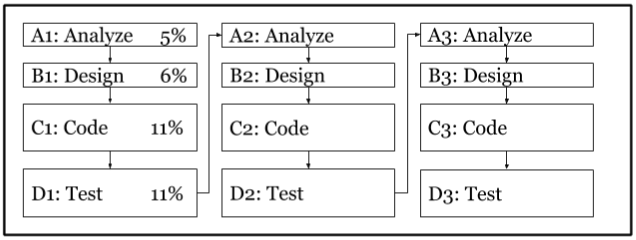
\includegraphics[scale=0.75]{iterative.png}
\end{center}

Assume that the total cost \& effort is the same for \ref{waterfall.tex} and \ref{iterative.tex}.
They differ only in how the SDLC is organized.


\quest{15 min}


\Q Based on the Iterative Model:

\begin{enumerate}%[itemsep=1ex]

\setlength{\defaultwidth}{15em}

\item How many stages are there?
\ans{12}

\item Which stage is 7th?
\ans{C2:~Code}

\item Which stages involve design?
\ans{B1, B2, B3}

\item What \% of total effort is for the \textbf{first four stages}?
\ans{33\% ~ A1+B1+C1+D1}

\item What \% of total effort is for \textbf{testing}?
\ans{33\% ~ D1+D2+D3}

\item What \% of total effort is for \textbf{analysis and design}?
\ans{33\% ~ A1+A2+A3 + B1+B2+B3}

\end{enumerate}


\Q Based on the Iterative Model:

\begin{enumerate}%[itemsep=1ex]

\setlength{\defaultwidth}{11em}

\item During what stage is the project \underline{25\%} completed?
\ans{D1}

\item When the project is \underline{25\%} completed, what \% of \textbf{analysis} is done?
\ans{33\% ~ A1 only}

\item When the project is \underline{25\%} completed, what \% of \textbf{coding} is done?
\ans{33\% ~ C1 only}

\item When the project is \underline{25\%} completed, what \% of \textbf{testing} is done?
\ans{About 9\% ~ (3\%/33\%)}

\item During what stage is the project \underline{50\%} completed?
\ans{C2}

\item When the project is \underline{50\%} completed, what \% of \textbf{analysis} is done?
\ans{67\% ~ A1 and A2}

\item When the project is \underline{50\%} completed, what \% of \textbf{coding} is done?
\ans{About 52\% ~ (17\%/33\%)}

\item When the project is \underline{50\%} completed, what \% of \textbf{testing} is done?
\ans{About 33\% ~ (11\%/33\%)}

\end{enumerate}


\vspace{1ex}
\comment{NOTE: The iterative model does not necessarily repeat exactly three times.
The key idea is that it repeats each stage multiple times, for the reasons you will identify on the next page.}

\newpage


\Q It is important to find and fix errors in software.

\begin{enumerate}%[itemsep=1ex]

\setlength{\defaultwidth}{8em}

\item If \textbf{analysis} errors are found during \textbf{A1:~Analyze}, \\ in which stage could they be fixed?
\ans{A1:~Analyze}

\item If \textbf{analysis} errors are found during \textbf{B1:~Design}, \\ in which stage could they be fixed?
\ans{A2:~Analyze}

\item If \textbf{coding} errors are found during \textbf{D2:~Test}, \\ in which stage could they be fixed?
\ans{C3:~Code}

\item If \textbf{analysis} errors are found during \textbf{B2:~Design}, \\ in which stage could they be fixed?
\ans{A3:~Analyze}

\item Are \textbf{analysis} errors likely to cause \textbf{design} errors?
\ans{Yes}

\item Are \textbf{design} errors likely to cause \textbf{coding} errors?
\ans{Yes}

\item Is it better to have \textbf{one try} or \textbf{several tries} \\ to remove all errors from the project?
\ans{several tries}

\end{enumerate}


\Q Explain why each test stage should try to find as many errors as possible.

\begin{answer}[5em]
The sooner you find a defect, (1) the easier it is to fix, and (2) the few other defects it causes.
\end{answer}


\Q Explain why \textbf{Iterative} is less likely then \textbf{Waterfall} to run into projects later in the project.

\begin{answer}[5em]
Iterative finds and fixes problems sooner, rather than waiting until the end of the life cycle.
\end{answer}
